\newcommand\tab[1][1cm]{\hspace*{#1}}
\graphicspath{{images/}{images/logos/}}
\begin{frame}{Unsere Aufgabe}
	Simulation des Festzuges in der Landshuter Innenstadt.
	Dabei sollen Menschen, Pferde und Kutschen in die Simulation eingebunden werden.
	Die Ergebnisse sollen schlußendlich für visuelle Darstellungen weiter gegeben werden.
	\newline \newline
	\underline{Simulations Tool:} \newline \tab OpenVadere (open source projekt) $\underline{}$
\end{frame}

\begin{frame}{Sprint Ziele}
	\begin{center}
		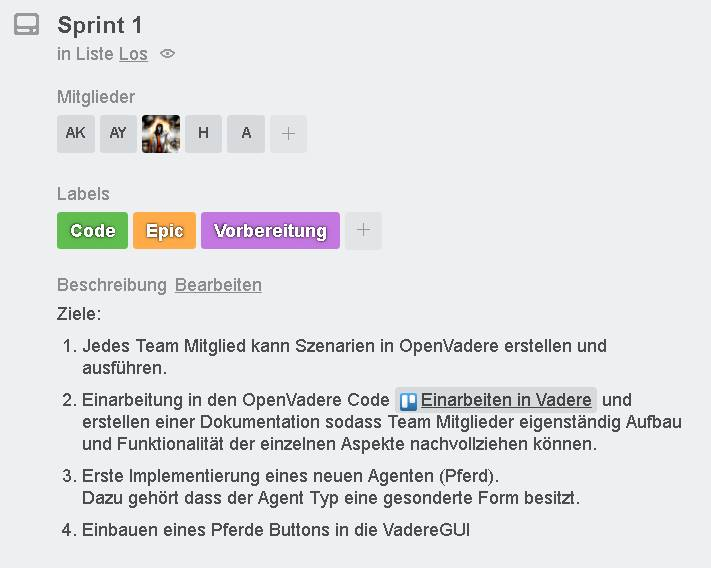
\includegraphics[width=260,height=240]{./sprint_goals.png}
	\end{center}
\end{frame}

\begin{frame}{Schwierigkeiten und Lösungen}
	\begin{itemize}
		\item Verstreutes Team \newline \tab Trello und Skype Calls
		\item Großes Projekt \& Wo anfangen?
			 \newline \tab Aufteilen des Teams auf die einzelnen Bereiche
			 \newline \tab Einarbeiten im Kontext eines neuen Agenten (Pferd)
	\end{itemize}
\end{frame}

\begin{frame}{Ausblick}
	\begin{itemize}
		\item Bewegungsmodel für Pferde einbinden.
		\item Schnittstelle zu den anderen Teams erweitern.
		\item Weitere Agententypes.
		\item Gui fertigstellen.
		\item Team:
			\begin{itemize}
				\item Code dojo
				\item Pair programming
			\end{itemize}
	\end{itemize}
\end{frame}
